% Szablon pracy dyplomowej Politechniki Łódzkiej (Zarządzenie 6/2025 Rektora PŁ)
\documentclass[W2, polski]{ThesisPLodz}

\authortitle{inż.}
\authorname{Neuro-Symbolic ADK}
\studentnumber{000000}
\boldauthorinbib{ADK, N.-S.}

\thesistitle{Automatyczna Synteza Systemów Neuro-Symbolicznych}
\thesisshorttitle{Synteza Systemów Neuro-Symbolicznych}

\degreename{magisterska}
\fieldofstudy{Sztuczna Inteligencja i Uczenie Maszynowe}
\department{Instytut Informatyki Stosowanej}

\supervisor{dr hab. inż. Promotor Akademicki, prof. PŁ}

\bibliographyfile{references}

\abstract{
Streszczenie w języku polskim opisujące motywację, formalną tezę badawczą, metodykę neuro-symboliczną oraz wyniki eksperymentów.
}
\keywords{sztuczna inteligencja, uczenie maszynowe, neuro-symbolic, optymalizacja}

\abstractsecondary{
Abstract in English presenting research thesis statement, architecture and empirical validation results.
}
\keywordssecondary{artificial intelligence, machine learning, neuro-symbolic AI, optimization}

\begin{document}

\chapter{Wstęp, Cel i Teza Pracy}
Rozdział wprowadzający z formalną tezą badawczą.

\chapter{Stan Wiedzy (SOTA)}
Przegląd literatury współczesnej (2023--2026).

\chapter{Architektura Systemu i Formalizm Matematyczny}
Opis architektury obliczeniowej z diagramem TikZ oraz stałymi AST:
\begin{table}[htbp]
\centering
\caption{Weryfikowane symbolicznie stałe konfiguracyjne}
\begin{tabular}{ll}
\toprule
\textbf{Symbol AST} & \textbf{Wartość w kodzie} \\
\midrule
LEARNING\_RATE & \texttt{\ref_ast{config.py:LEARNING_RATE}} \\
\bottomrule
\end{tabular}
\end{table}

\begin{figure}[htbp]
\centering
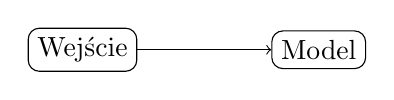
\begin{tikzpicture}
  \node[draw, rectangle, rounded corners] (a) {Wejście};
  \node[draw, rectangle, rounded corners, right of=a, node distance=3cm] (b) {Model};
  \draw[->] (a) -- (b);
\end{tikzpicture}
\caption{Architektura systemu.}
\label{fig:arch_tikz}
\end{figure}

\chapter{Implementacja Algorytmiczna}
Opis realizacji algorytmu w module \texttt{core.py}.

\chapter{Badania Eksperymentalne i Wyniki}
Tabela wyników empirycznych z wskaźnikami \texttt{\textbackslash ref\_csv}:
\begin{figure}[htbp]
\centering
\includegraphics[width=0.86\textwidth]{figures/comparison_chart.pdf}
\caption{Porównanie wyników eksperymentalnych.}
\label{fig:comparison_chart}
\end{figure}

\chapter{Podsumowanie i Wnioski}
Podsumowanie i weryfikacja postawionej tezy.

\bibliographystyle{plain}
\bibliography{references}

\symbolslist{
  $\eta$ -- współczynnik uczenia \\
  $\mathcal{L}$ -- funkcja straty
}

\abbreviationslist{
  PŁ -- Politechnika Łódzka \\
  ADK -- Artificial Degree Printer Development Kit
}

\definitionslist{
  Neuro-Symbolic AI -- paradygmat łączący reprezentację wiedzy i sieci neuronowe.
}

\end{document}

